\chapter{基于CAE-CNN的无线信号调制识别}

\section{引言}

无线通信领域的研究人员已经开始将深度神经网络应用于认知无线电,并取得了一定的成果[13] [12][10]。
[Tim Oshea]最近证明了利用原始数据进行有监督无线调制识别[14]的可行性,
作者利用原始信号经希尔伯特变换后得到的$I$与$Q$路信号作为训练样本,调制方式作为标签,训练CNN分类器。
结果显示,其分类性能超越了传统的基于专家特征的决策树、SVM等分类模型。
然而,作者仅仅是用了传统的CNN框架,并没有对分类性能以及网络框架进行进一步的研究。\par

本章针对无线信号调制识别问题,提出了一种基于卷积自编码器(CAE)与卷积神经网络(CNN)融合的无线信号调制识别的算法框架,
并将此框架下的识别准确率及鲁棒性等与传统的基于特征的识别方法进行比较分析。\par

\section{调制信号生成}

无线接收端的信号实际上是信号经过信道作用得到的。
尽管在机器学习中我们一般会建议使用真实数据,但是在无线电通信领域中,
由于标记数据匮乏,而且受到多径等效应的影响,很难直接使用真实数据进行训练。
我们利用XXX仿真仪,构建通信系统框架,通过多径信道和高斯信道来获取近似真实的仿真信号。\par

\subsection{调制信号获取}
% 为了简化信号的生成,我们使用XXX信号生成器自带的信道模型,这包括许多所需的信道,例如高斯信道,频率选择性信道、多径信道、瑞利信道等。下文当中使用的数据,我们是利用高斯信道生成的数据。\par

无线通信信号实际上是经过调制信号与信道综合作用生成的。
我们以与真实系统完全相同的方式确定性地引入调制,脉冲整形,携带数据以及与现实通信系统相同的发射参数。 
我们将真实的语音和文本数据集调制到信号上,这样,接收信号不仅是一系列的确知信号,并且包含了信息,
使我们的调制信号更接近真实环境中的信号。\par

信号源我们使用XXX信号发生器生成随机信号,然后加入高斯白噪声,并对基带信号进行调制。
信道我们分别使用高斯信道和多径信道进行仿真,由于高斯信道过于理想,
为了更好地还原现实世界中信道对调制信号的影响,我们最终使用的数据是基于多径信道仿真的生成信号。\par

随后,我们使用XXX频谱分析仪对经过多径信道后的样本进行采样,获取原始的IQ两路采样数据。
由于数据本身是一个很长的时间序列,并不适合后期的分类器学习。
因此,我们使用128个样本大小的滑动窗口,在采样信号序列上滑动,每次移动64个样本,来获取训练样本。
最后利用python的pickle包将其持久化到本地文件,每个样本以32位浮点数的复数形式保存,总数据集大约600MB。\par

XXX信号发生器的系统参数如表\ref{sec:table_3_0}所示:\par
\begin{table}[H]
	\centering
	\caption{系统参数配置}
	\begin{tabular}{ccc}
		\toprule
		参数 & 配置\\
		\midrule
		System & Ubuntu 17.10\\
		\bottomrule
	\end{tabular}
	\label{sec:table_3_0}  
\end{table}

我们的采样率大约为1M/sec,则每一个样本的持续时间约为128μs。每个样本大约包含8到16个符号,它们含有经过信道带来的随机时间偏移,缩放,旋转,相位和噪声等。\par
整个调制信号生成的系统框图如图\ref{sec:fig_3_1}所示。\par
\begin{figure}
	\centering
	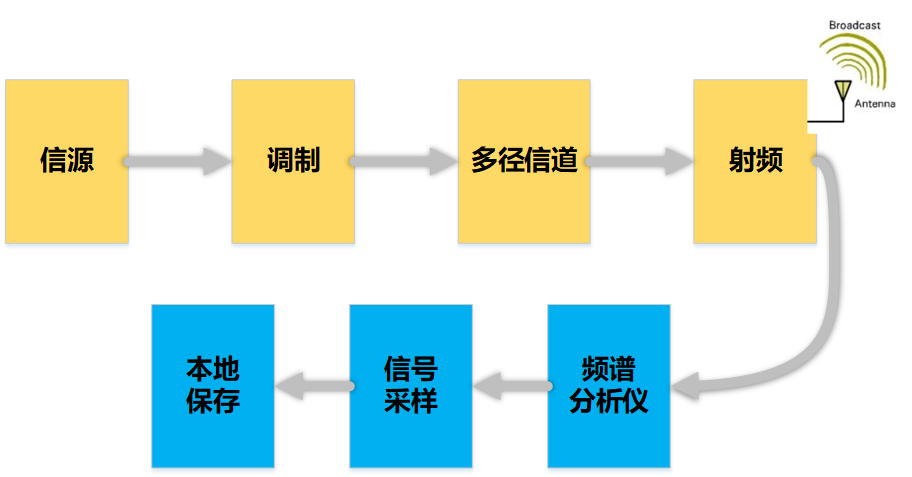
\includegraphics[scale=0.6]{./figures/chapter_3/fig_3_1}
	\caption{调制信号生成框图}\label{sec:fig_3_1}
\end{figure}
最后,我们生成的数据集主要由9种调制方式组成:8类数字调制和1类模拟调制,这些都被广泛应用于我们周围的无线通信系统。
这些调制类别包括BPSK,QPSK,8PSK,16QAM,64QAM,BFSK,CPFSK和PAM4等数字调制方式,以及用于模拟调制的AM-DSB。 
数据以大约每个符号8次采样的速率进行采样,数据源的平均发送功率为0dB。\par


\section{调制信号的表示}

不同的调制信号具有不同的时频特征。本节,我们将原始数据可视化,了解不同信号的时频特征;
同时,我们利用CAE以及CNN获取信号的无监督表示,并展示不同信号在CAE特征空间中的分布状况,
从而进一步了解不同网络框架对调制信号进行特征提取的不同状况。

\subsection{数据集可视化}

对于每一种调制方式,我们随机抽出一个样本,并对其时域(图\ref{sec:fig_3_1})和频域(图\ref{sec:fig_3_2})进行展示。
我们可以发现,不同调制方式之间具备许多相似性,同事也具备一定差异性。有些信号我们是可以通过肉眼进行模糊判别;
但是,受脉冲形变,失真和其他信道影响,有些信号即便是人类专家也很难从视觉上分辨属于何种调制类别。\par

如图(图\ref{sec:fig_3_2})所示,在时域中,我们可以看到XX信号具备较明显的特征,
而XXX特征在视觉上让人感觉像是噪声,很难直接判断出来。\par

\begin{figure}[!h]
	\centering
	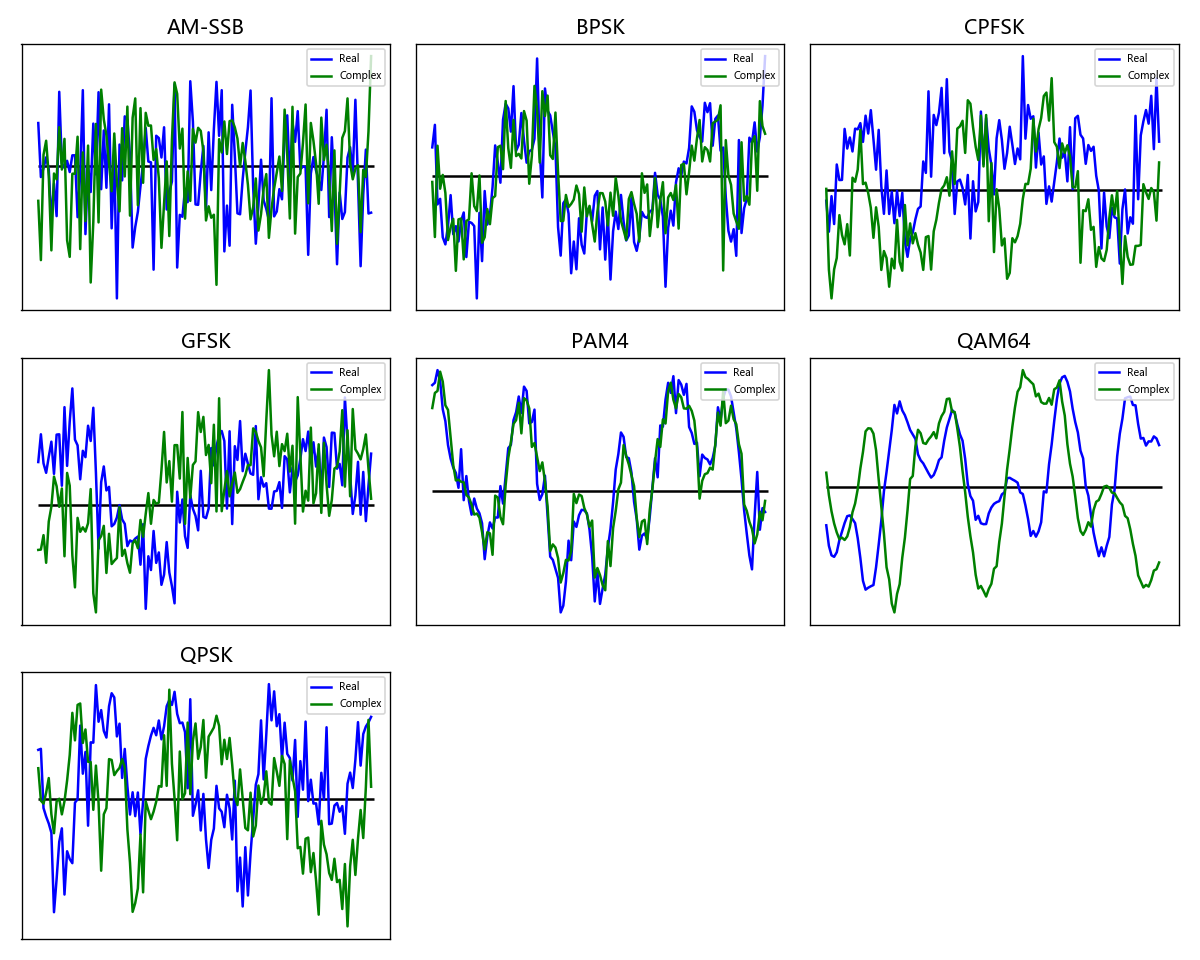
\includegraphics[scale=0.3]{figures/chapter_3/fig_3_2}
	\caption{不同调制方式的高SNR样本的时域波形}\label{sec:fig_3_2}
\end{figure}

如图(图\ref{sec:fig_3_3})所示,在频域中,每一个信号都具备一个带宽限制的功率包络,
其形状为调制识别提供了一定的信息,但是对于人类专家来说,从视觉来区分不同的调制信号是一个困难且繁琐的判定方法。\par
\begin{figure}[!h]
	\centering
	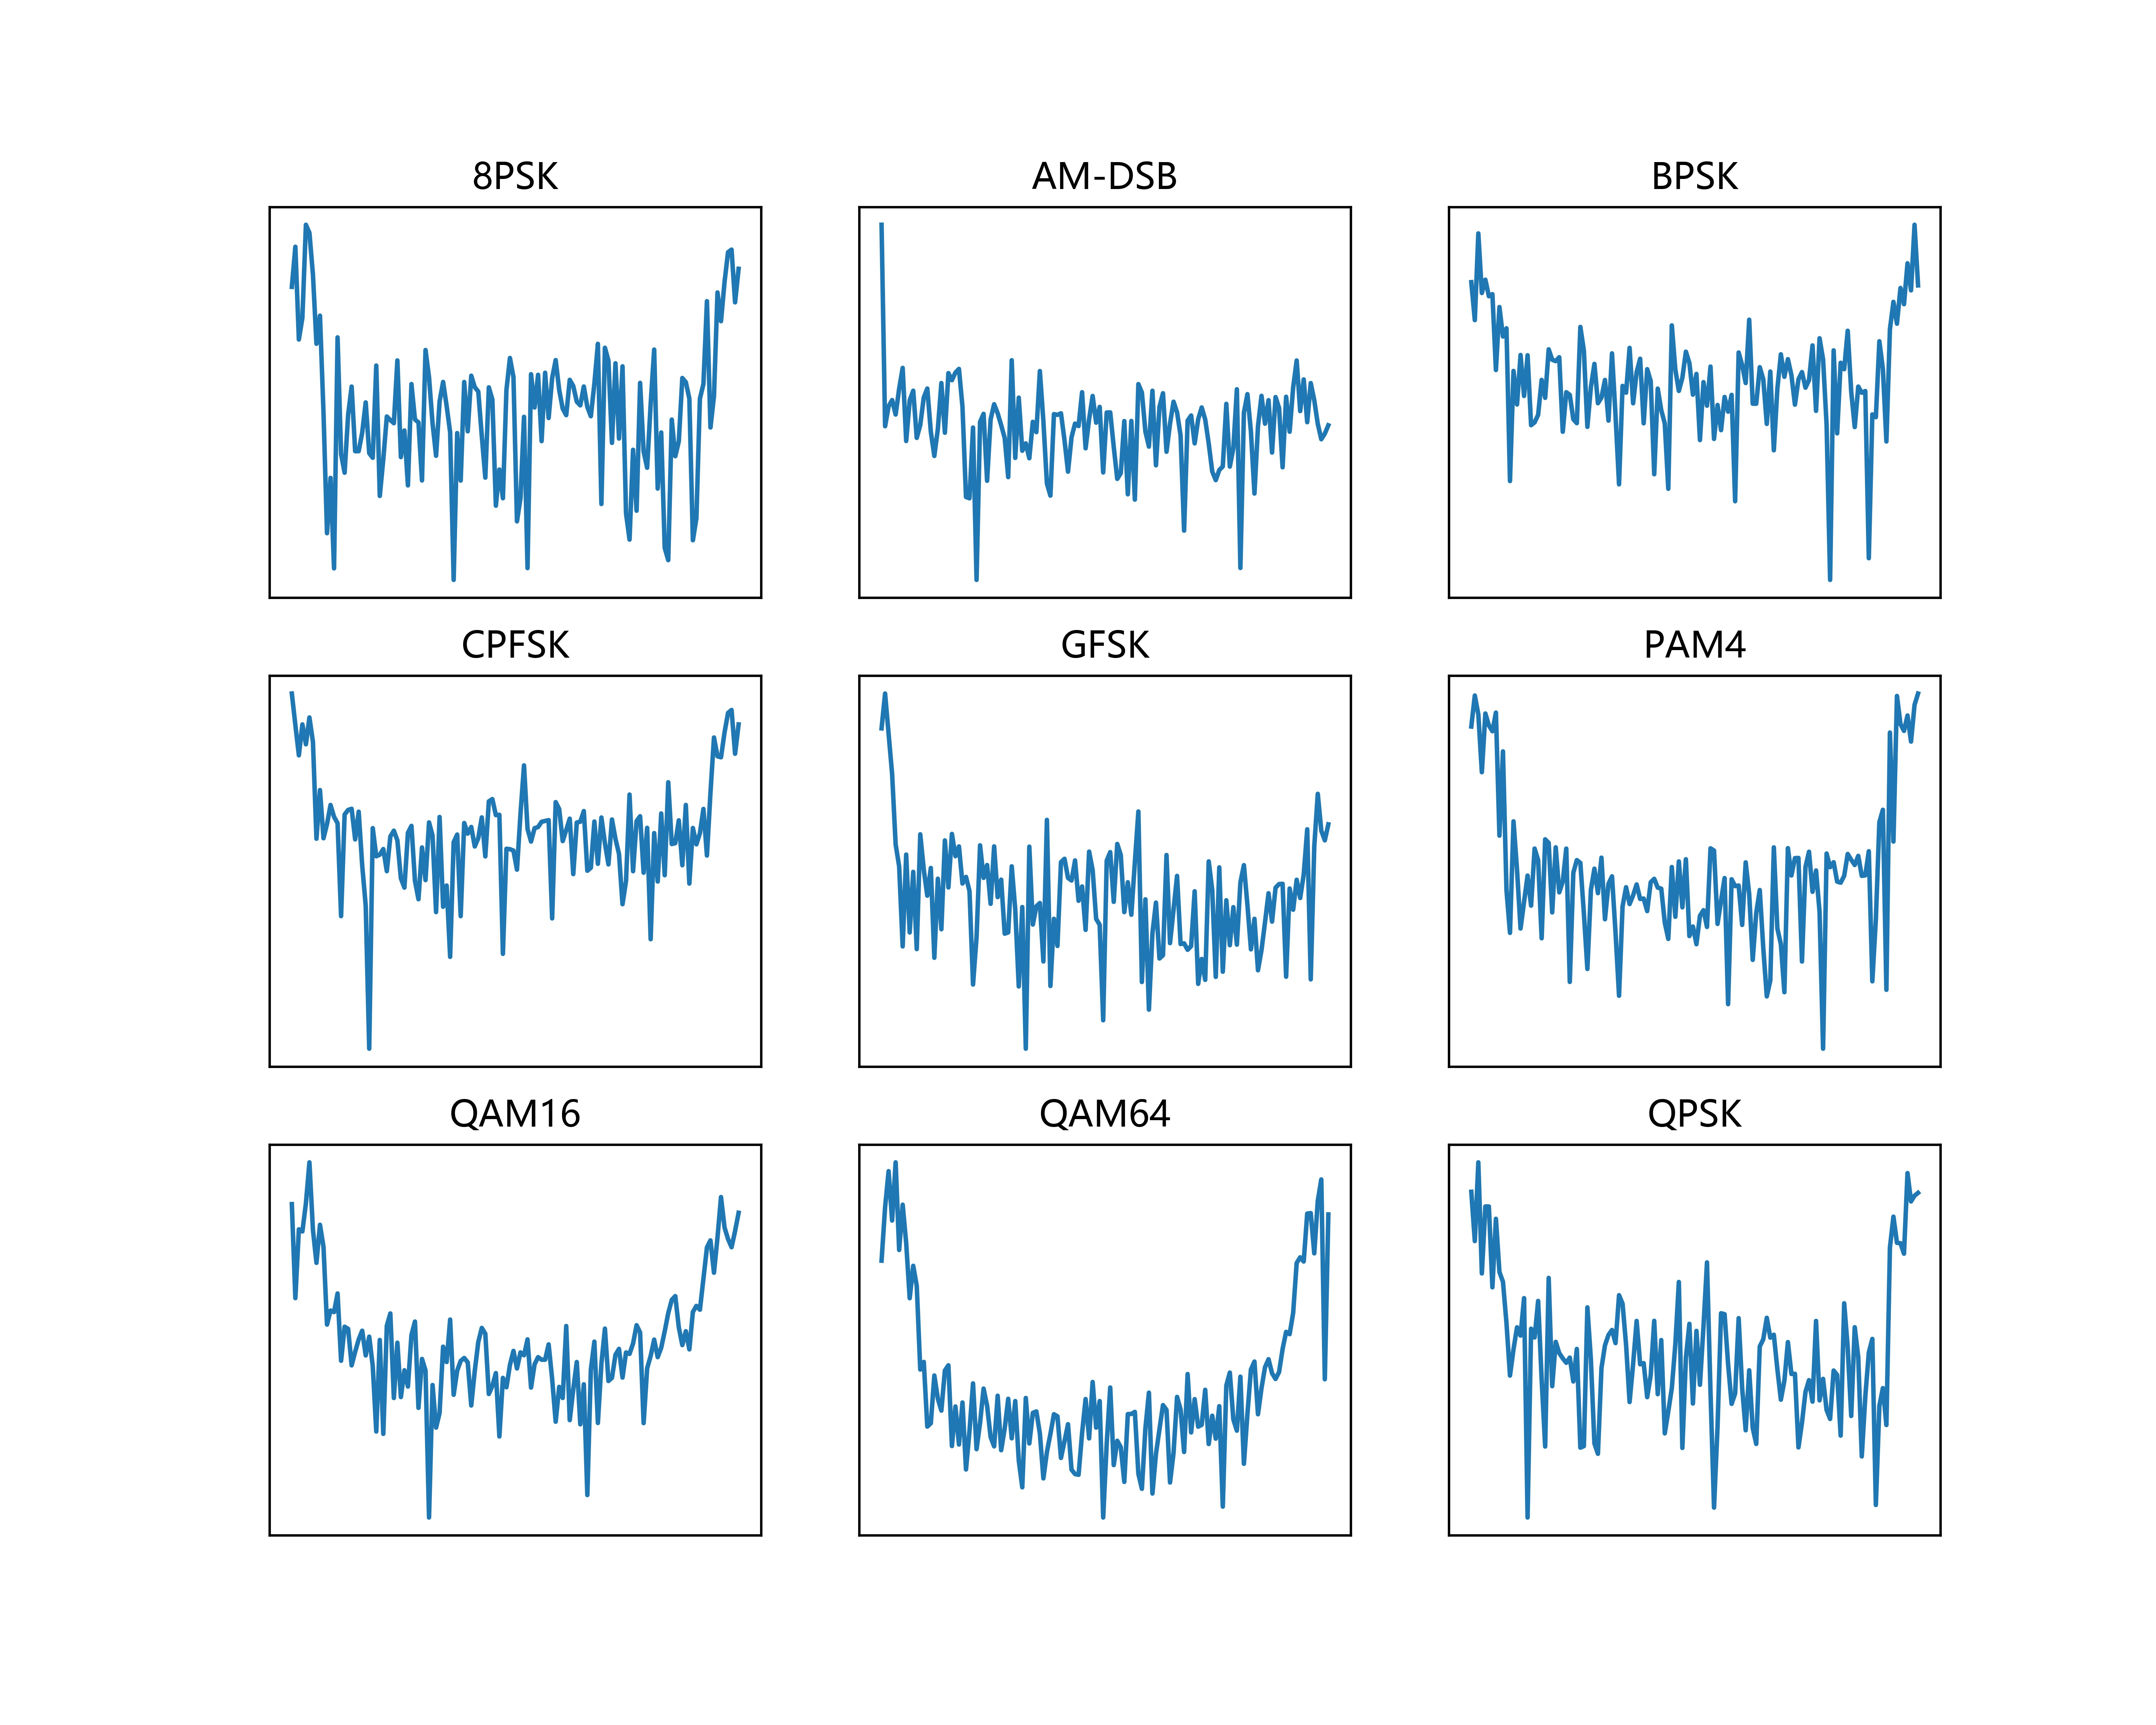
\includegraphics[scale=1.0]{figures/chapter_3/fig_3_3}
	\caption{不同调制方式的高SNR样本的频谱}\label{sec:fig_3_3}
\end{figure}


\subsection{调制信号的无监督表示}

无监督的稀疏表示是指在没有使用类标签的情况下,利用无监督的方法来学习数据集的稀疏表示。
这可以通过使用基于数据依赖性的降维技术来完成,例如主成分分析(PCA)或独立分量分析(ICA)。
但是,这些方法只能对数据进行线性降维,如果说处于低维流型的数据与原始空间本身不具备线性关系,
那么这种情况下就不适合使用线性降维方法。\par

卷积自动编码器(Convolutional Autoencoder,CAE)非常适合于减小参数空间,获取的卷及特征具有时移不变性。
在CAE的训练过程中,我们尽量减少信号重构的均方误差(MSE),但由于我们的主要目标是获得原始信号的聚类稀疏表示,
因此我们对重构误差作出简化假设:限制重构误差最小的情况下尽量降低隐藏层的维度。
然而,由于很难确定重构误差的最小值,
所以,我们只能人为的指定隐层的维度来确定我们的稀疏表示维度,在维度确定的情况下调整参数使重构误差尽量小。
本文中,我们利用卷积自编码器对输入的信号进行重构,学习一组原始信号的非线性稀疏表示。\par

自动编码器是一种无监督的学习算法,其中神经网络的优化目标是通过一些更有约束的中间维度,使用均方误差(MSE)等损失函数,最小化输出处的重构误差。通常,自编码器利用反向传播算法,将误差进行反向传播,并使用随机梯度下降(SGD)算法等,以找到接近等式\ref{sec:eqt_3_1}中的最佳网络参数。

\begin{equation}\label{sec:eqt_3_1}
	\mathop{\arg\min}_{\theta}(\sum(X − f (X,\theta))^2)
\end{equation}

通过约束网络的中间层维度,从而可以通过提取用于聚类的中间稀疏编码,来获得原始数据的非线性降维。在这种情况下,使用相似的调制信号,可以由相似的卷积核和特征图来表示,因此,他们分布在该压缩空间的相近区域中。自编码器中的卷积层具有时移不变性以及受约束的参数搜索空间(相对于全连接层),因此非常适合于无线电时间序列信号表示。我们使用dropout[13]并在输入层加入噪声[7]对网络进行正则化,来增强模型的泛化能力。图\ref{sec:fig_3_4}显示了我们的卷积自动编码器使用的体系结构。\par

\begin{figure}[!h]
	\centering
	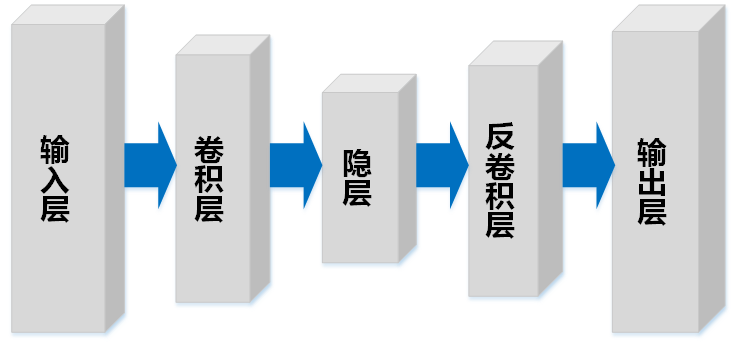
\includegraphics[scale=0.6]{figures/chapter_3/fig_3_4}
	\caption{自编码器}	\label{sec:fig_3_4}
\end{figure}

我们使用RMSProp[11]和Adam[12]梯度下降求解器进行优化,两者都获得了相似的结果,
下文中我们默认使用具备自适应学习速率的Adam优化器进行训练。\par

图\ref{sec:fig_3_5}显示了两个输入维度为$2x128$的训练样本,中间隐层维度为$1x30$,
以及输出维度为$2x128$的训练结果展示图。\par
\begin{figure}[!h]
	\centering
	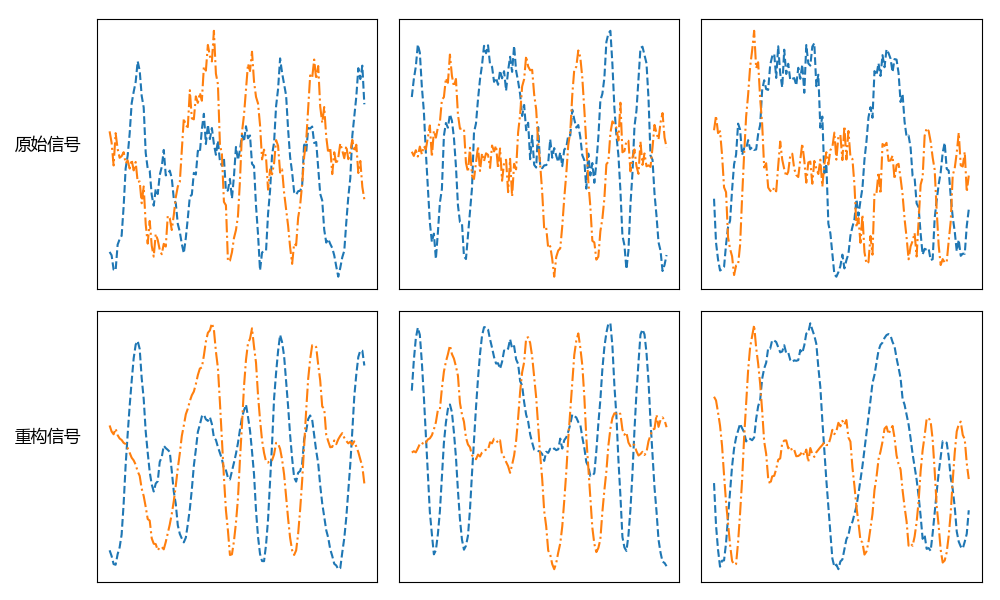
\includegraphics[scale=0.2]{figures/chapter_3/fig_3_5}
	\caption{基于自编码器的信号复现}	\label{sec:fig_3_5}
\end{figure} 

通过图\ref{sec:fig_3_5},我们可以发现,卷积自编码器可以很好的复现原始信号;
我们提取的特征可以很好地重构原始数据,即可以很好地表征原始数据。
这说明我们的卷积自编码器可以通过无监督的方式学习信号的低维嵌入表示。\par

为了可视化我们学到的卷及特征,并对这些特征的类可分性进行直观展示,我们将数据的低维嵌入特征,
利用t-分布随机邻接嵌入(t-asdfasdfa,t-SNE)[6]算法映射到二维流型,并在平面坐标系中展示。
在低维嵌入空间中分布在相近的区域的样本,分布在二维流型中相近的区域。
因此,我们可以通过观察不同类别的数据样本在t-SNE可视化之后的二维流型上的分布,来反映样本无监督表示的类可分性。\par

我们训练卷积自编码器从每一类样本中随机采样100个样本,将其通过训练的卷积自编码器获得其低维无监督表示,
并利用t-SNE映射到二维流型,最终的效果如图X:

\begin{figure}[!h]
	\centering
	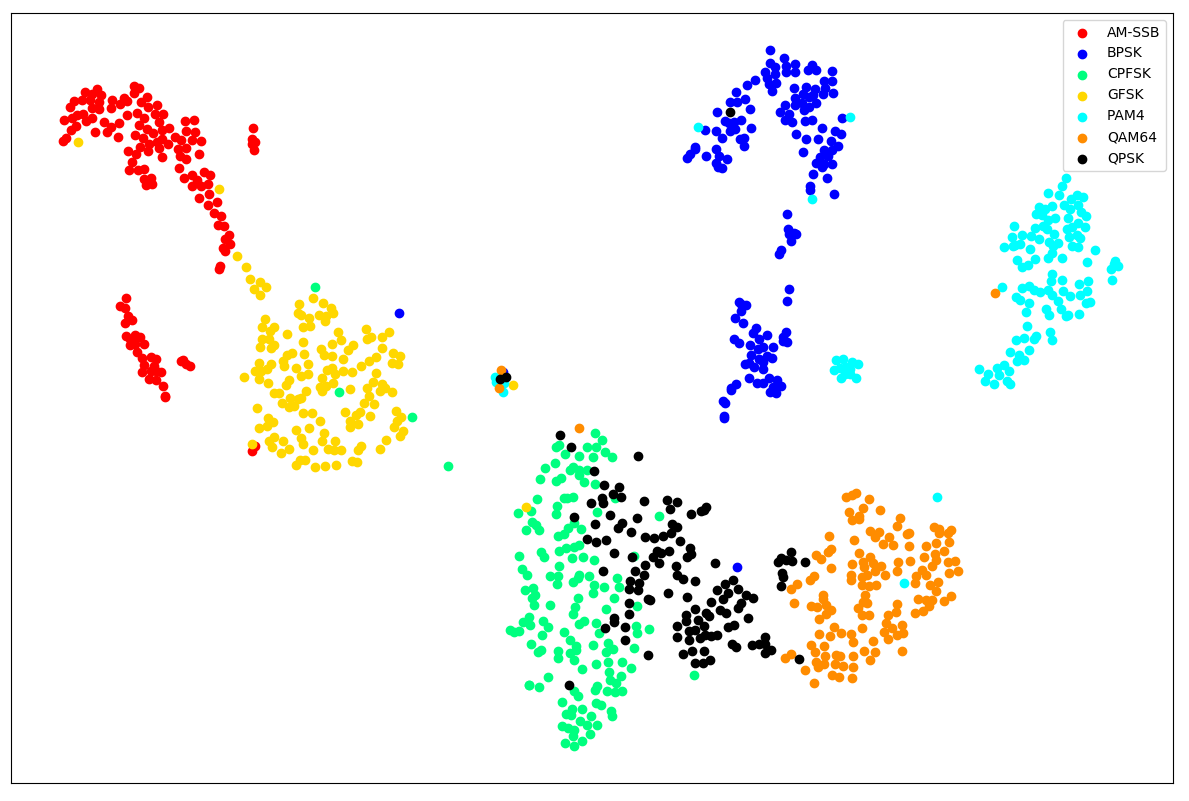
\includegraphics[scale=0.4]{figures/chapter_3/fig_3_6}
	\caption{基于自编码器的调制信号large-vis二维流型展示}	\label{sec:fig_3_6}
\end{figure}

在这种情况下,我们看到几个类如WBFM,AMDSB, AM-SSB和QPSK已经形成了独立的、大部分可分离的簇,
可以利用DBSCAN等聚类方法形成单独的类别;而其他类则会出现类别混淆,并且难以通过聚类方法分离类别簇。 
尽管我们的无监督表示类可分性效果不是很好,但考虑到这些特征从来没有被训练用来区分不同类别的样本,
我们就已经获得了数据一定程度的类可分性,这已经算是一个可以接受的结果了。 \par 

\subsection{调制信号的监督引导稀疏表示}

当我们具有一部分监督数据的时候,我们也可以使用监督训练时学习到的判别特征生成一个稀疏表示空间。
TIM Shead在他的工作[14]中,利用有标记样本以监督方式训练卷积神经网络,可以达到很好的分类效果。
CNN主要是由卷基层与DNN层构成;由于CNN本身可以对测试样本进行分类,这就相当于在进行Softmax层的分类之前,
我们已经获取了原始数据具有类别区分度的特征。
因此,我们可以利用监督的方式,获取原始数据的监督引导特征。\par

在训练好分类网络以后,我们移除最后的softmax层,保留剩余的这一部分网络。
这样,在样本经过训练好的网络,最后隐层输出的特征即为原始数据的稀疏表示。
我们利用监督方式训练网络,并获取监督引导特征空间,获取数据监督引导的稀疏表示。\par
我们从每一类样本中随机采样100个样本,通过图X的网络将其映射到监督引导特征空间,并利用t-SNE映射到二维流型,最终的效果如图X:
\begin{figure}[!h]
	\centering
	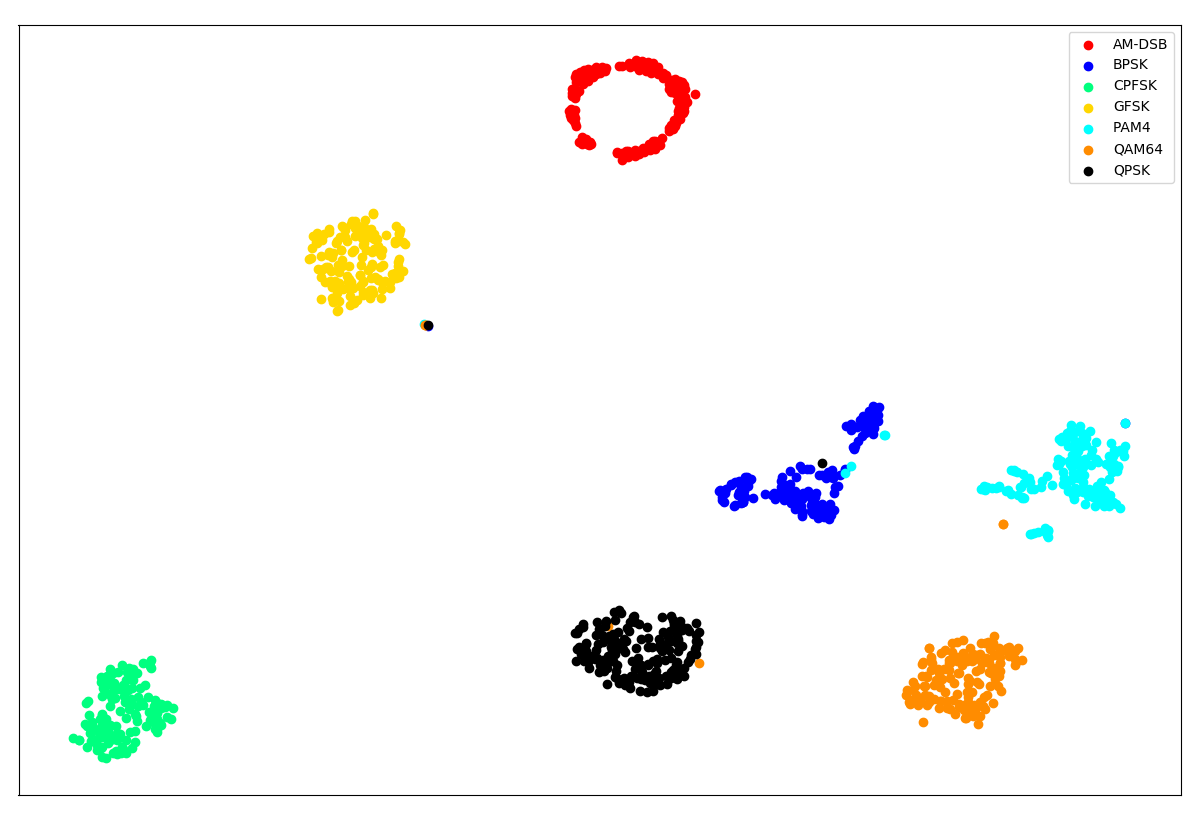
\includegraphics[scale=0.4]{figures/chapter_3/fig_3_7}
	\caption{基于CNN的调制信号large-vis二维流型展示码器}	\label{sec:fig_3_7}
\end{figure}

在这种情况下,我们几乎可以把每个调制类别的样本在二维流型中利用聚类算法分开。
当然,其中也有一部分的数据是混淆的,比如类别X中也有部分样本散落到类别X中。\par
可能是因为在获取监督引导特征空间时,我们的目标是正确区分不同的调制类别,
所以我们获取的监督引导特征对于不同类别的样本是有一定的区分度的,即不同调制类别的样本分布在特征空间的不同区域,
这就表现为在t-SNE之后不同类别样本分布在二维流型的不同区域。
当然,随着训练网络时样本类别的增加,我们获取的具有类区分度的特征将会得到更好的泛化。\par


\section{基于CAE-CNN的无线信号调制识别}

在上一节中,我们分别使用监督引导和无监督引导的方法获取数据的低维表示,其本质上就是基于降维的非线性特征提取过程。
在本节中,通过融合CAE与CNN,我们联合重构误差与分类误差,提出了一种新的调制识别网络框架和算法。

\subsection{CAE-CNN网络框架}
在上一节中,我们发现数据样本在低维嵌入空间中的表示具有一定的类可分性。因此,我们可以将CNN分为特征提取与分类两个步骤。
对于CAE与CNN的融合,我们的本质是希望能够在分类的同时保证特征提取尽量多地包含数据的原始信息。
为此,我们通过在CNN的交叉熵损失中加入CAE的重构误差损失作为我们的整体损失;
通过改进CAE与CNN的训练算法,降低重构误差与分类误差,达到更好的分类效果。
图\ref{sec:fig_3_8}展示了我们网络的结构:

\begin{figure}[!h]
	\centering
	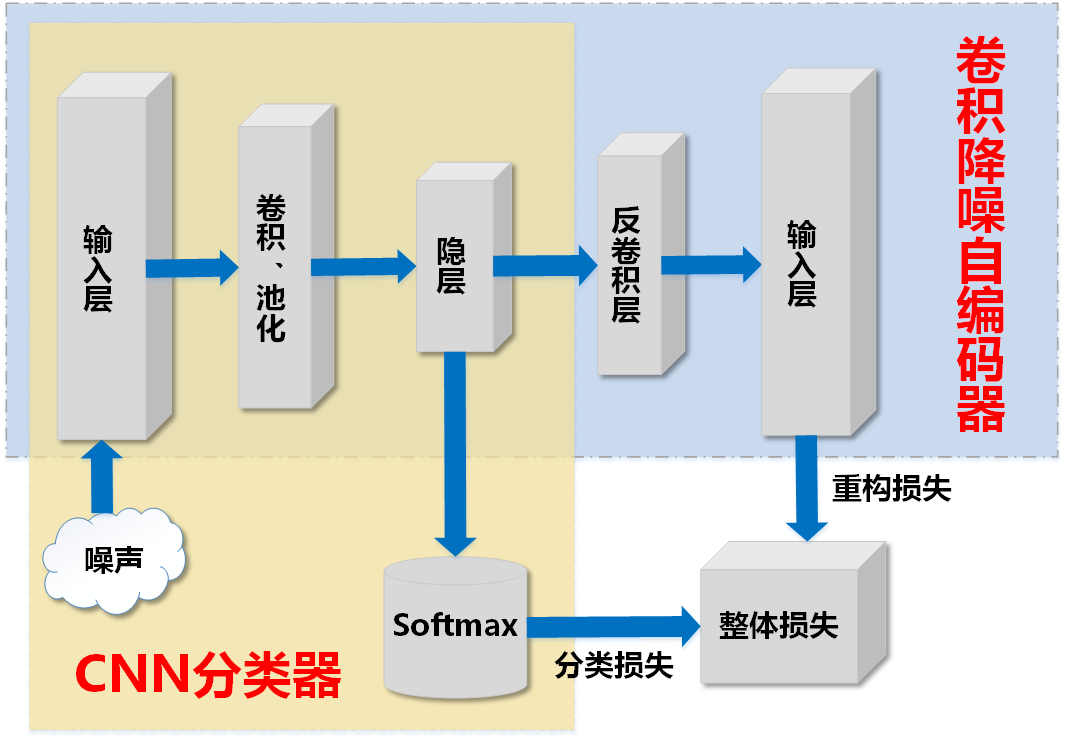
\includegraphics[scale=0.5]{figures/chapter_3/fig_3_8}
	\caption{CAE-CNN网络框架}	\label{sec:fig_3_8}
\end{figure}

在CAE-CNN中的卷基层中,我们使用了Dropout,用以降低模型的过拟合影响;
并在卷积权重增加了权重值$W$的2范数作为惩罚项,使权重尽量小;
同时,我们在第一个密集连接层加入权重的$F1$范数范数惩罚来鼓励解的稀疏性[5][10]。\par

那么我们有CAE的损失函数:
\begin{equation}\label{sec:eqt3_3}
r(t) = s(t)*c + n(t)
\end{equation}

由于CNN的损失函数为重构误差与分类误差之和,那么我们有CNN的损失函数:
\begin{equation}\label{sec:eqt3_4}
r(t) = s(t)*c + n(t)
\end{equation}

\subsection{CAE-CNN算法}

\begin{algorithm}[ht]
	\caption{CAE-CNN算法}
	\label{alg:CAE_CNN}
	\begin{algorithmic}
		\REQUIRE 步长 $\epsilon$ (建议默认为: $0.001$)
		\REQUIRE 矩估计的指数衰减速率, $\rho_1$ 和 $\rho_2$ 在区间 $[0, 1)$内。
		(建议默认为:分别为$0.9$ 和 $0.999$)
		\REQUIRE 用于数值稳定的小常数 $\delta$  (建议默认为: $10^{-8}$)
		\REQUIRE 初始参数 $\theta$
		\STATE 初始化一阶和二阶矩变量 $s = 0 $, $r = 0$
		\STATE 初始化\gls{time_step} $t=0$ 
		\WHILE{没有达到停止\gls{criterion}}
		\STATE 从\gls{training_set}中采包含$m$个样本$\{ x^{(1)},\dots, x^{(m)}\}$ 的\gls{minibatch},对应目标为$y^{(i)}$。
		\STATE 计算梯度:$g \leftarrow \frac{1}{m} \nabla_{\theta} \sum_i L(f(x^{(i)};\theta),y^{(i)})$ 
		\STATE $t \leftarrow t + 1$
		\STATE 更新有偏一阶矩估计: $s \leftarrow \rho_1 s + (1-\rho_1) g$
		\STATE 更新有偏二阶矩估计:$r \leftarrow \rho_2 r + (1-\rho_2)  g \odot g$
		\STATE 修正一阶矩的\gls{bias_sta}:$\hat{s} \leftarrow \frac{s}{1-\rho_1^t}$
		\STATE 修正二阶矩的\gls{bias_sta}:$\hat{r} \leftarrow \frac{r}{1-\rho_2^t}$
		\STATE 计算更新:$\Delta \theta = - \epsilon \frac{\hat{s}}{\sqrt{\hat{r}} + \delta}$ \ \  (逐元素应用操作)
		\STATE 应用更新:$\theta \leftarrow \theta + \Delta \theta$
		\ENDWHILE
	\end{algorithmic}
\end{algorithm}


\subsection{算法运行环境及参数}
使用分类交叉熵损失函数和Adam[15]求解器进行训练(在我们的数据集上略胜过RMSProp[12])。
我们在tensorflow[16]计算框架上运行网络的训练和预测,使用Nvidia NVIDIA Cuda[8]组件,
在Nvidia GTX1080ti显卡上加速运算。接下来的仿真我们都使用这一套软硬件组合进行仿真。
我们的机器系统配置如表\ref{sec:table_3_1}所示:\par

\begin{table}[H]
	\centering
	\caption{系统参数配置}
	\begin{tabular}{ccc}
		\toprule
		参数 & 配置\\
		\midrule
		System & Ubuntu 17.10\\
		\midrule
		CPU & Intel\textsuperscript{\textregistered}  Xeon(R) CPU E5-2683 v3 \\
		\midrule
		GPU & GeForce GTX 1080 Ti\\
		\midrule 
		Memory & 64GB\\
		\midrule 
		HardDisk & 1TB\\
		\midrule 
		Python & python3.6\\
		\midrule 
		Library & Tensorflow1.4\\
		\bottomrule
	\end{tabular}
	\label{sec:table_3_1}  
\end{table}

\section{结果及分析}

\subsection{学习复杂度}
我们使用Adam求解器训练了大约23分钟的最高复杂度模型,批量大小为1024的样本训练集大约需要15秒。我们确实观察到一些过度拟合,尽管没有正规化,但验证损失确实 没有显着变化,我们保持最佳的验证损失模型进行评估。\par

绘制学习的特征有时可以让我们直觉了解网络正在学习的底层表示。 在这种情况下,我们在下面绘制卷积层1和卷积层2的滤波器权重。 在图5中,第一层,我们有64个1x3的过滤器。 在这种情况下,我们只需获得一组边缘和梯度检测器,它们在每个I和Q通道上进行操作。\par

在卷积层2中,如图6所示的权重,我们将这个第一层特征图组合成64×16×2×3较大的特征图,其包括在I和Q通道上同时出现的情况。 这些特征图与在包括2D学习边缘检测器和Gabor滤波器的图像转换网络的较低层处所看到的特征图看起来没有太大的不同。\par

\subsection{分类准确率与鲁棒性}
\subsubsection{分类结果}
为了评估分类器的性能,我们看一下测试数据集的分类性能。
我们调制方式总共有11中,每一类调制信号在噪声信噪比为$-20dB~18dB$之间每隔$2dB$进行数据采样,
每个信噪比下采样1000个样本,每个样本共包含128个采样值;
我们将采样值进行希尔伯特变化,这样每个采样值便分为实部与虚部。
我们将80\%的样本作为训练集,10\%的样本作为验证集集,10\%的样本作为测试集。
即训练样本大约有。 这些样本均匀分布在从-20dB到+ 20dB的SNR中,并被标记以便我们可以评估特定子集上的性能。\par
\begin{figure}[!h]
	\centering
	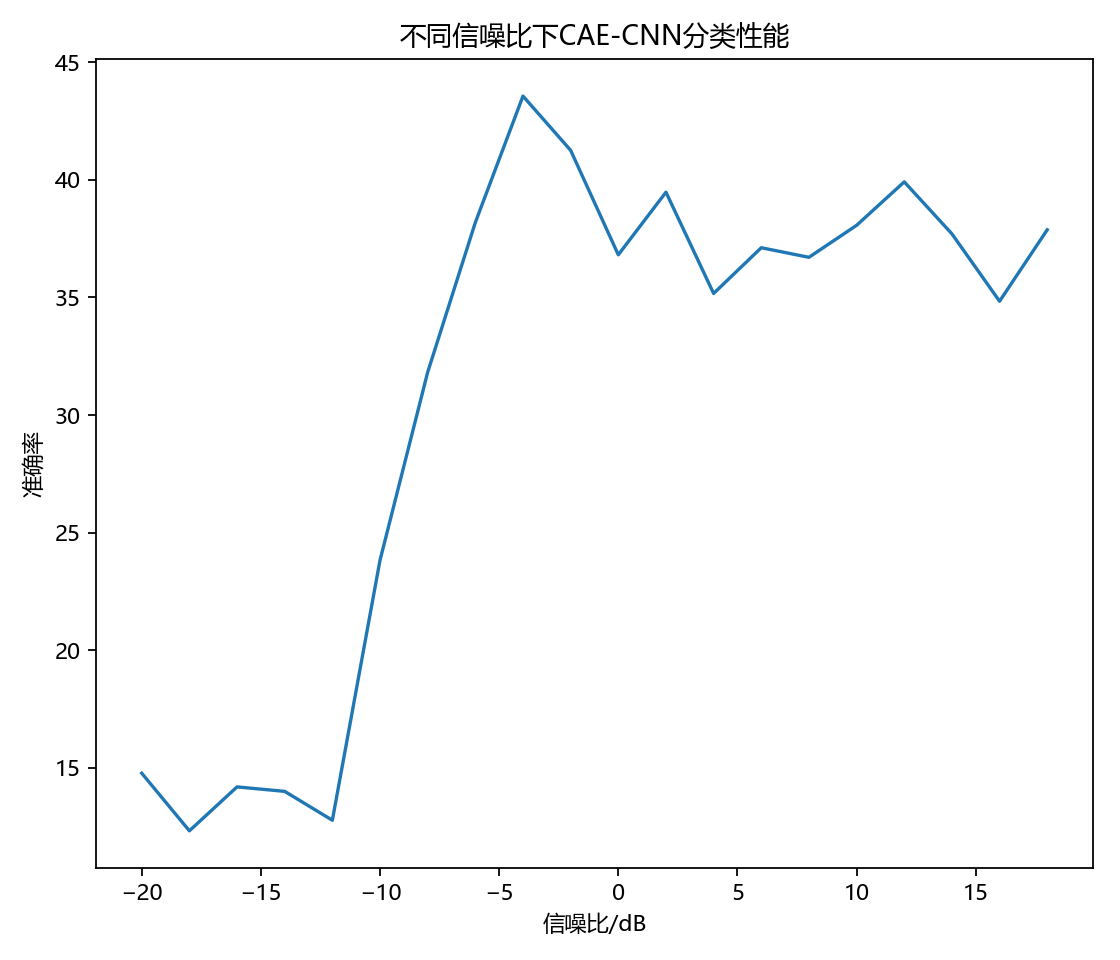
\includegraphics[scale=0.7]{figures/chapter_3/fig_3_9}
	\caption{整体结果}	\label{sec:fig_3_9}
\end{figure}
对于我们最高的SNR情况下的CNN2(0.6)分类,我们在图8中显示了一个混淆矩阵。在+18dBSNR时,在混淆矩阵中我们有一个干净的对角线,可以看到我们剩下的差异是8PSK误分类为QPSK,WBFM误分类作为AM-DSB。这两个都可以在基础数据集中解释。由于QPSK星座点由8PSK点跨越,所以包含特定比特的8PSK符号从QPSK难以分辨。在WBFM /AM-DSB的情况下,模拟语音信号具有只有载波音调存在的静默时段,这使得这些示例不可见。因此,即使在这个数据集的高信噪比下,也不可能获得100%的准确度,并使得重新合理的混淆被合理地容忍。\par
\subsubsection{0dB误分结果}
\begin{figure}[!h]
	\centering
	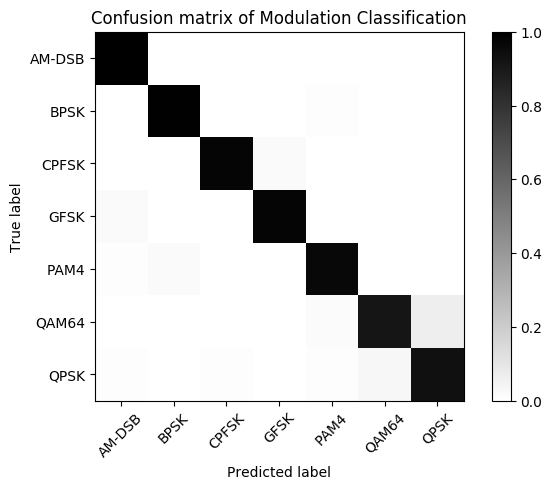
\includegraphics[scale=0.8]{figures/chapter_3/fig_3_10}
	\caption{0dB条件下的结果}	\label{sec:fig_3_10}
\end{figure}

\subsubsection{与其他算法的比较}
\begin{figure}[!h]
	\centering
	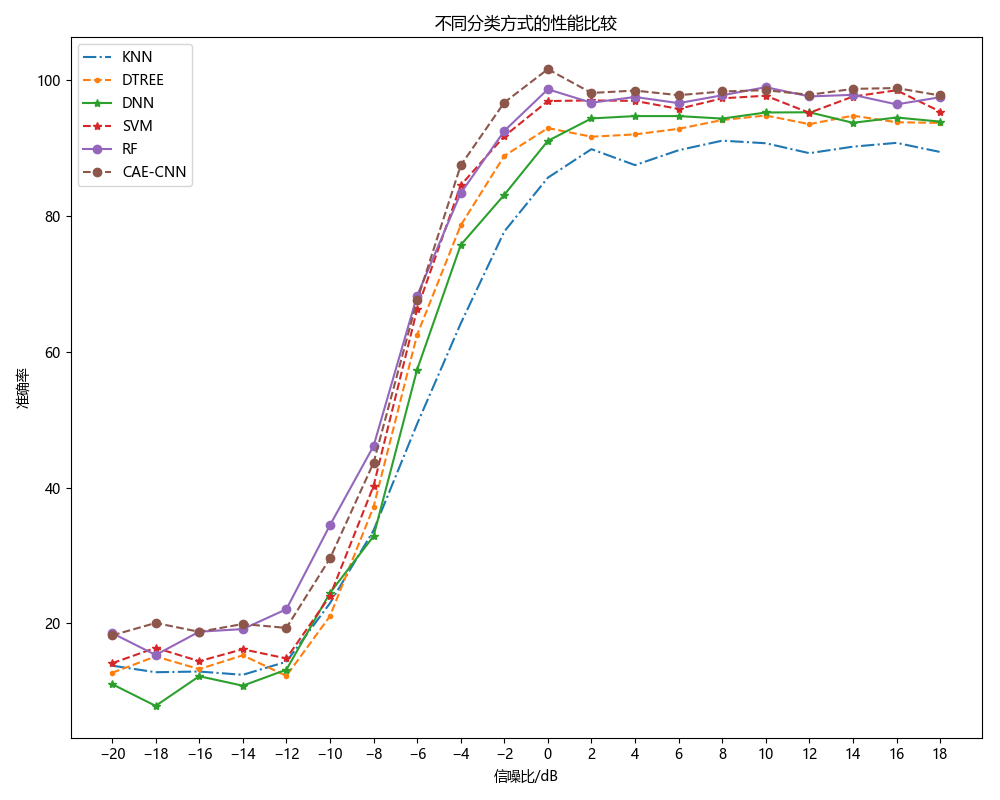
\includegraphics[scale=0.6]{figures/chapter_3/fig_3_11}
	\caption{与其他方法的比较}	\label{sec:fig_3_11}
\end{figure}

在训练之后,我们在测试数据集上的所有信噪比之间的分类准确率大致达到了87.4%,但要理解这个意义,我们必须检查这个分类精度如何在不同训练样本的SNR值之间进行分解,以及 它与现有的基于专家特征的分类器的性能进行比较。绘制测试集调制分类精度,作为每个分类器的示例信噪比的函数7。 实线表示直接在无线电时间序列数据上进行深度特征学习训练的分类器,而虚线表示使用前面描述的专家特征作为输入的分类器。 这种观点是检验结果的关键方法,因为在低信噪比影响范围和覆盖范围的性能,我们可以有效地使用分类器。 我们从具有大量丢失正则化(0.6)的大卷积神经网络(CNN2)中获得显着更好的低SNR分类准确性性能。 在低信噪比情况下,最佳CNN模型的性能比基于专家特征的系统的信噪比高2.5-5dB,而+ 5dB SNR性能相似。 这是一个显着的性能改进,可能至少是传感系统有效覆盖面积的两倍。\par


\subsection{训练效率以及分类效率}

a)训练时间
\begin{figure}[!h]
	\centering
	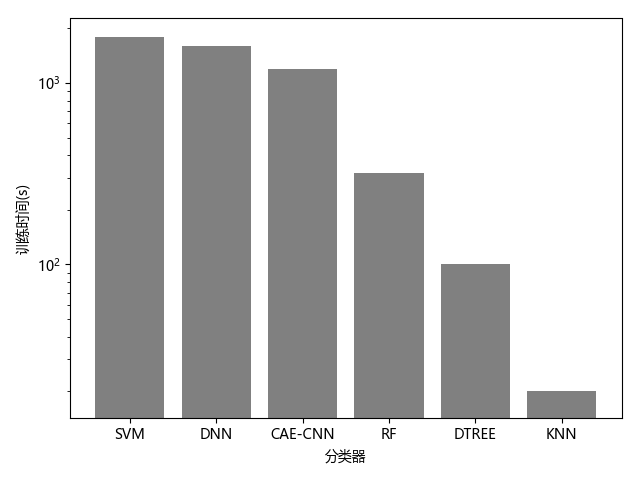
\includegraphics[scale=0.7]{figures/chapter_3/fig_3_12}
	\caption{训练时间}	\label{sec:fig_3_12}
\end{figure}

为了更好地理解性能如何随信噪比而变化,我们检查了不同信噪比级别的几个分类器的混淆矩阵。\par

在非常低的信噪比(-6dB)的情况下,在图9,10,11和12中,我们看到一个有趣的情况,其中±20%内的所有精度都在50%左右。在这种情况下,CNN2分类器上的清洁器对角线比其他3种情况显着更明显,在这个区域学习到的特征具有显着的性能优势。\par

现在,所有4个分类器的信噪比(0dB)略高但仍然很低,现在有一个明确的对角线,但是我们发现在8PSK情况下发生的非对角线误分类更少。\par

b)分类时间

许多无线电系统中的一个重要考虑因素是训练和分类运行时间,由于计算复杂性。 深度学习的一个普遍批评是对大量计算资源的需求,然而在本文中,我们的网络相对紧凑,数据集相对较小。 我们比较下面每个模型的训练和分类运行时间。 在图17中我们可以看到,我们的CNN模型确实需要大量的训练时间,但是比SVM训练案例所需要的时间要少。\par
\begin{figure}[!h]
	\centering
	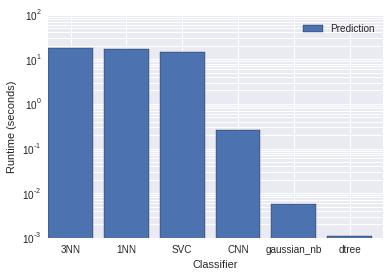
\includegraphics[scale=0.7]{figures/chapter_3/fig_3_13}
	\caption{分类时间}	\label{sec:fig_3_13}
\end{figure}

在图18中显示,使用Tensorflow编译python的这个模型的分类时间比使用scikit-learn的最近邻和SVM模型的大多数其他模型显着更快。只有决策树和GaussianNB模型获得更快的分类运行时间。在这两种情况下,基于ConvNet的这种规模的这种数据集分类模型提出了一个有吸引力的选择这个任务时,分类性能考虑。\par


\section{本章小结}

一旦示例在嵌入空间中形成相对可分的簇,我们可以使用任意数量的聚类算法来将它们中的每一个分组并将其分配给类标签。在图9中,我们展示了一个使用DBSCAN [4]聚类算法的例子,将聚类分成一组未知但不同的调制类。我们发现这种聚类方法比较适合在我们的压缩空间中形成的不明确形状的聚类。聚类之后的数据处理可以包括标记许多示例的集群而不是每个单独的示例,从而提供从数据保存时间的效率提高的数量级。在包含许多类和例子的非常大的数据集上,这使得管理大规模学习任务比其他方法更容易处理。\par
虽然这些集群并非没有错误,但是在这个例子中,通常我们可以找到从发现的类集合到不同的真实命名类的一对一或多对一的映射。这保证了这样一种方法可以在将来用于快速组织和标记大量的无线电发射,并利用关于发射器类别特征的先前知识,但是仍然允许随着时间的推移识别系统能力,特征和类别标签的缩放最大限度地减少这样做所需的人力劳动。\par

虽然这些结果并不是现有的最好的基于专家特征的调制分类器的全面比较,但是它们证明了,与相对专业的被认为的方法相比,时间序列无线电信号数据上的盲卷积网络是可行的并且工作得很好。在图7中,我们比较了几种分类器策略的准确性和信噪比,并且认为对于低信噪比和短时间的示例(128个复杂采样),这代表了调制分类的最先进的精确度方法。这种方法有可能容易地扩展到额外的调制类别,并且应该被视为依赖于无线电发射器的稳健的低SNR分类的DSA和CR系统的有力候选。\par


我们的结果与当前最好的专家系统方法的合理近似相比较,但是由于在无线电领域新兴的机器学习领域不存在强大的竞争数据集,所以很难直接比较性能和当前的现有技术状态。我们希望在以后的工作中进一步评估这一点,并将特征学习和专家方法从目前的水平上进行改进。 CNN2网络体系结构上的性能改进是不可避免的,我们花费了一些努力来优化它,但并没有做到这一点。较大的过滤器,不同的体系结构和池化层可能会显着影响性能,但是在这项工作中没有充分考虑其适用性。许多附加技术可以应用于这个问题,包括引入附加通道引起的效应的不变性,例如膨胀,I / Q不平衡,相位偏移等等。空间变换网络[17]已经证明了学习图像数据的这种不变性的强大能力,并且可以作为一个有趣的候选者,使得能够改善对这些效应的不变性学习。序列模型和递归层[13]可能能够表示信号序列嵌入,并且在更长时间表示中几乎肯定会证明是有价值的,但是我们还没有完全调查这个区域。这个应用领域已经成熟,可以进一步研究和应用,这将大大影响无线信号处理和认知无线电领域的技术发展水平,并将其转向机器学习和数据驱动方法。\par

